\documentclass{llncs}

\usepackage{graphicx}
\usepackage{rotating}
\usepackage{verbatim}
\usepackage{url}
%\usepackage[square]{natbib}

\title{Designing a Search Application for the British Broadcasting Corporation (BBC) Using UML}
\author{Ross Fenning\inst{1}
  \and Huseyin Dogan\inst{2}
  \and Keith Phalp\inst{2}}
\institute{BBC, UK \email{Ross.Fenning@bbc.co.uk}
  \and Bournemouth University, UK \email{\{hdogan,kphalp\}@bournemouth.ac.uk}}

\begin{document}

\maketitle

\begin{abstract}

Whilst there are successful general web search engines such as Google that
will find any piece of content, there is a perceived need for a specific
search that makes better use of the internal knowledge the broadcasting
industry (e.g. BBC) has about its own content. The British Broadcasting
Corporation (BBC) is a public service broadcaster funded by the licence
fee paid by United Kingdom households. This industry-based case study
looks at the applicability of Soft Systems Methodology (SSM) and
Unified Modelling Language (UML) to design a hypothetical, high-level
view of a search application that receives
web content from a variety of BBC content production systems and makes
every item then searchable by a BBC website visitor using the search
feature. The developers of such search applications can benefit from this
specific industry-based case study that contextualised the problem space
using SSM and developed UML models to solve the problem.

\end{abstract}

\section{The Problem}

\subsection{Background}

The BBC has been publishing content on the World Wide Web since the
mid 1990s and since then the amount and the diversity has increased
exponentially. Large websites -- or indeed the web as a whole --
would not have been usable nor useful without the rise in quality of
web search engines.

A large challenge for any web search application is to provide a common
interface and set of user interactions that can equally index, search
and link to a diverse range of types of information -- be it in the form
of text, images, video or games. A more recent challenge has been to
achieve this in a near-real time way to catch up with the rapid rate at
which content is added to the web (particulary from microblogging websites
such as Twitter).

Whilst there are successful general web search engines such a Google that
will find any piece of content, there is a perceived need for a
BBC-specific search that makes better use of the internal knowledge the BBC
has about its own content.

\subsection{Problem Space Contextualisation through Soft Systems}

The purpose of this paper is to start the high-level design -- and
look at the lower levels of one or two aspects -- of a search application
specific to BBC content. The intent is to provide a consistent user interface
that allows the audience to find news articles, sport results,
TV catch-up, education resources and everything else the BBC produces.

Whilst the BBC website currently has a
functional search feature already, this paper assumes building a new search application
from the ground up so as to give full freedom to apply the analysis and design
techniques therein. In practice, there are engineering challenges involved
in maintaining and building on top of existing systems. Such challenges
are out of scope for this paper.

The target audience for the BBC is effectively the entire population of the UK
and amongst those that do make use of BBC services, there is much diversity
of needs, preferences and technical ability. It is clear it is no small
task to design a search-based discovery mechanism of millions of diverse
pieces of content aimed at millions of diverse people.

Using \emph{Soft Systems Methodology} (SSM)
\cite{checkland2006learning}, we can stand back from
an ontological approach of defining what the search system \emph{is} or
\emph{comprises} and instead take an \emph{epistemological} view of search
as a system. With this view, we could consider a system that holistically
transforms members of the public's desires to find online content into
the consumption of that content -- whether those desires are \emph{precise}
(e.g. they want an exact article known by headline they saw earlier or a
particular programme they missed on television) or those desires are
\emph{fuzzy} (e.g. news about a certain topic, any comedy programme, learning
materials about the Industrial Revolution).

Checkland and Scoles\cite{checkland1990soft} decribed a \emph{Rich Picture} approach
for representing a problem situation early in SSM approaches.
Given the size and complexity of the
search system as a whole, a useful initial step is to create such an informal
representation of what is known about the problem. Figure~\ref{rich-picture}
shows what the authors know of the audience, search and most BBC online content areas.
Note that not all areas are covered and a strong emphasis is placed on TV
catch-up (e.g. via the iPlayer product). Radio catch-up is not mentioned
as it shares a lot of similarity with television in terms of use and any
differences are out of scope for this design.

Dogan and Henshaw\cite{dogan2010transition}
showed how a ``soft'' systems approach called Interactive
Management can be adopted to capture the requirements and contextualise the
problem space. This involved the process of transitioning from the soft systems
results to a formal model (e.g. UML). This transition was enabled by dividing
the actors in the rich pictures into meta-level and direct users of the system.
Although this division was subjective and depended on the interpretation  and
analysis of the rich pictures to provide a structure for the use case model,
the rich pictures themselves were created through interactions with subject
matter experts. The soft systems, and hence the Interactive Management results,
provided the baseline information to derive a formal model including UML use
case, sequence and domain models. The transitioning from ``soft'' to ``hard''
systems can be set within the State of the Art including the requirements
analysis and modelling as used in SSM, UML and Business Process Modelling.

The overall design objective of this paper will be to create an initial
proposal for a
search application to drive the missing components within the holistic
system depicted in Fig.~\ref{rich-picture}. Some subsystems already
exist, e.g. for journalists to write news articles and publish them on the
BBC News website, but for the purposes of this design exercise, we will
assume no existing application to drive a search-based discovery of
those websites.

The design will look to integrate with
existing subsystems where possible rather than attempt to replicate
work already done. For example, journalists will prefer that a search
application can integrate with the system into which they are publishing
their articles instead of being required to publish their articles into
two systems.

\begin{sidewaysfigure}
  \begin{center}
    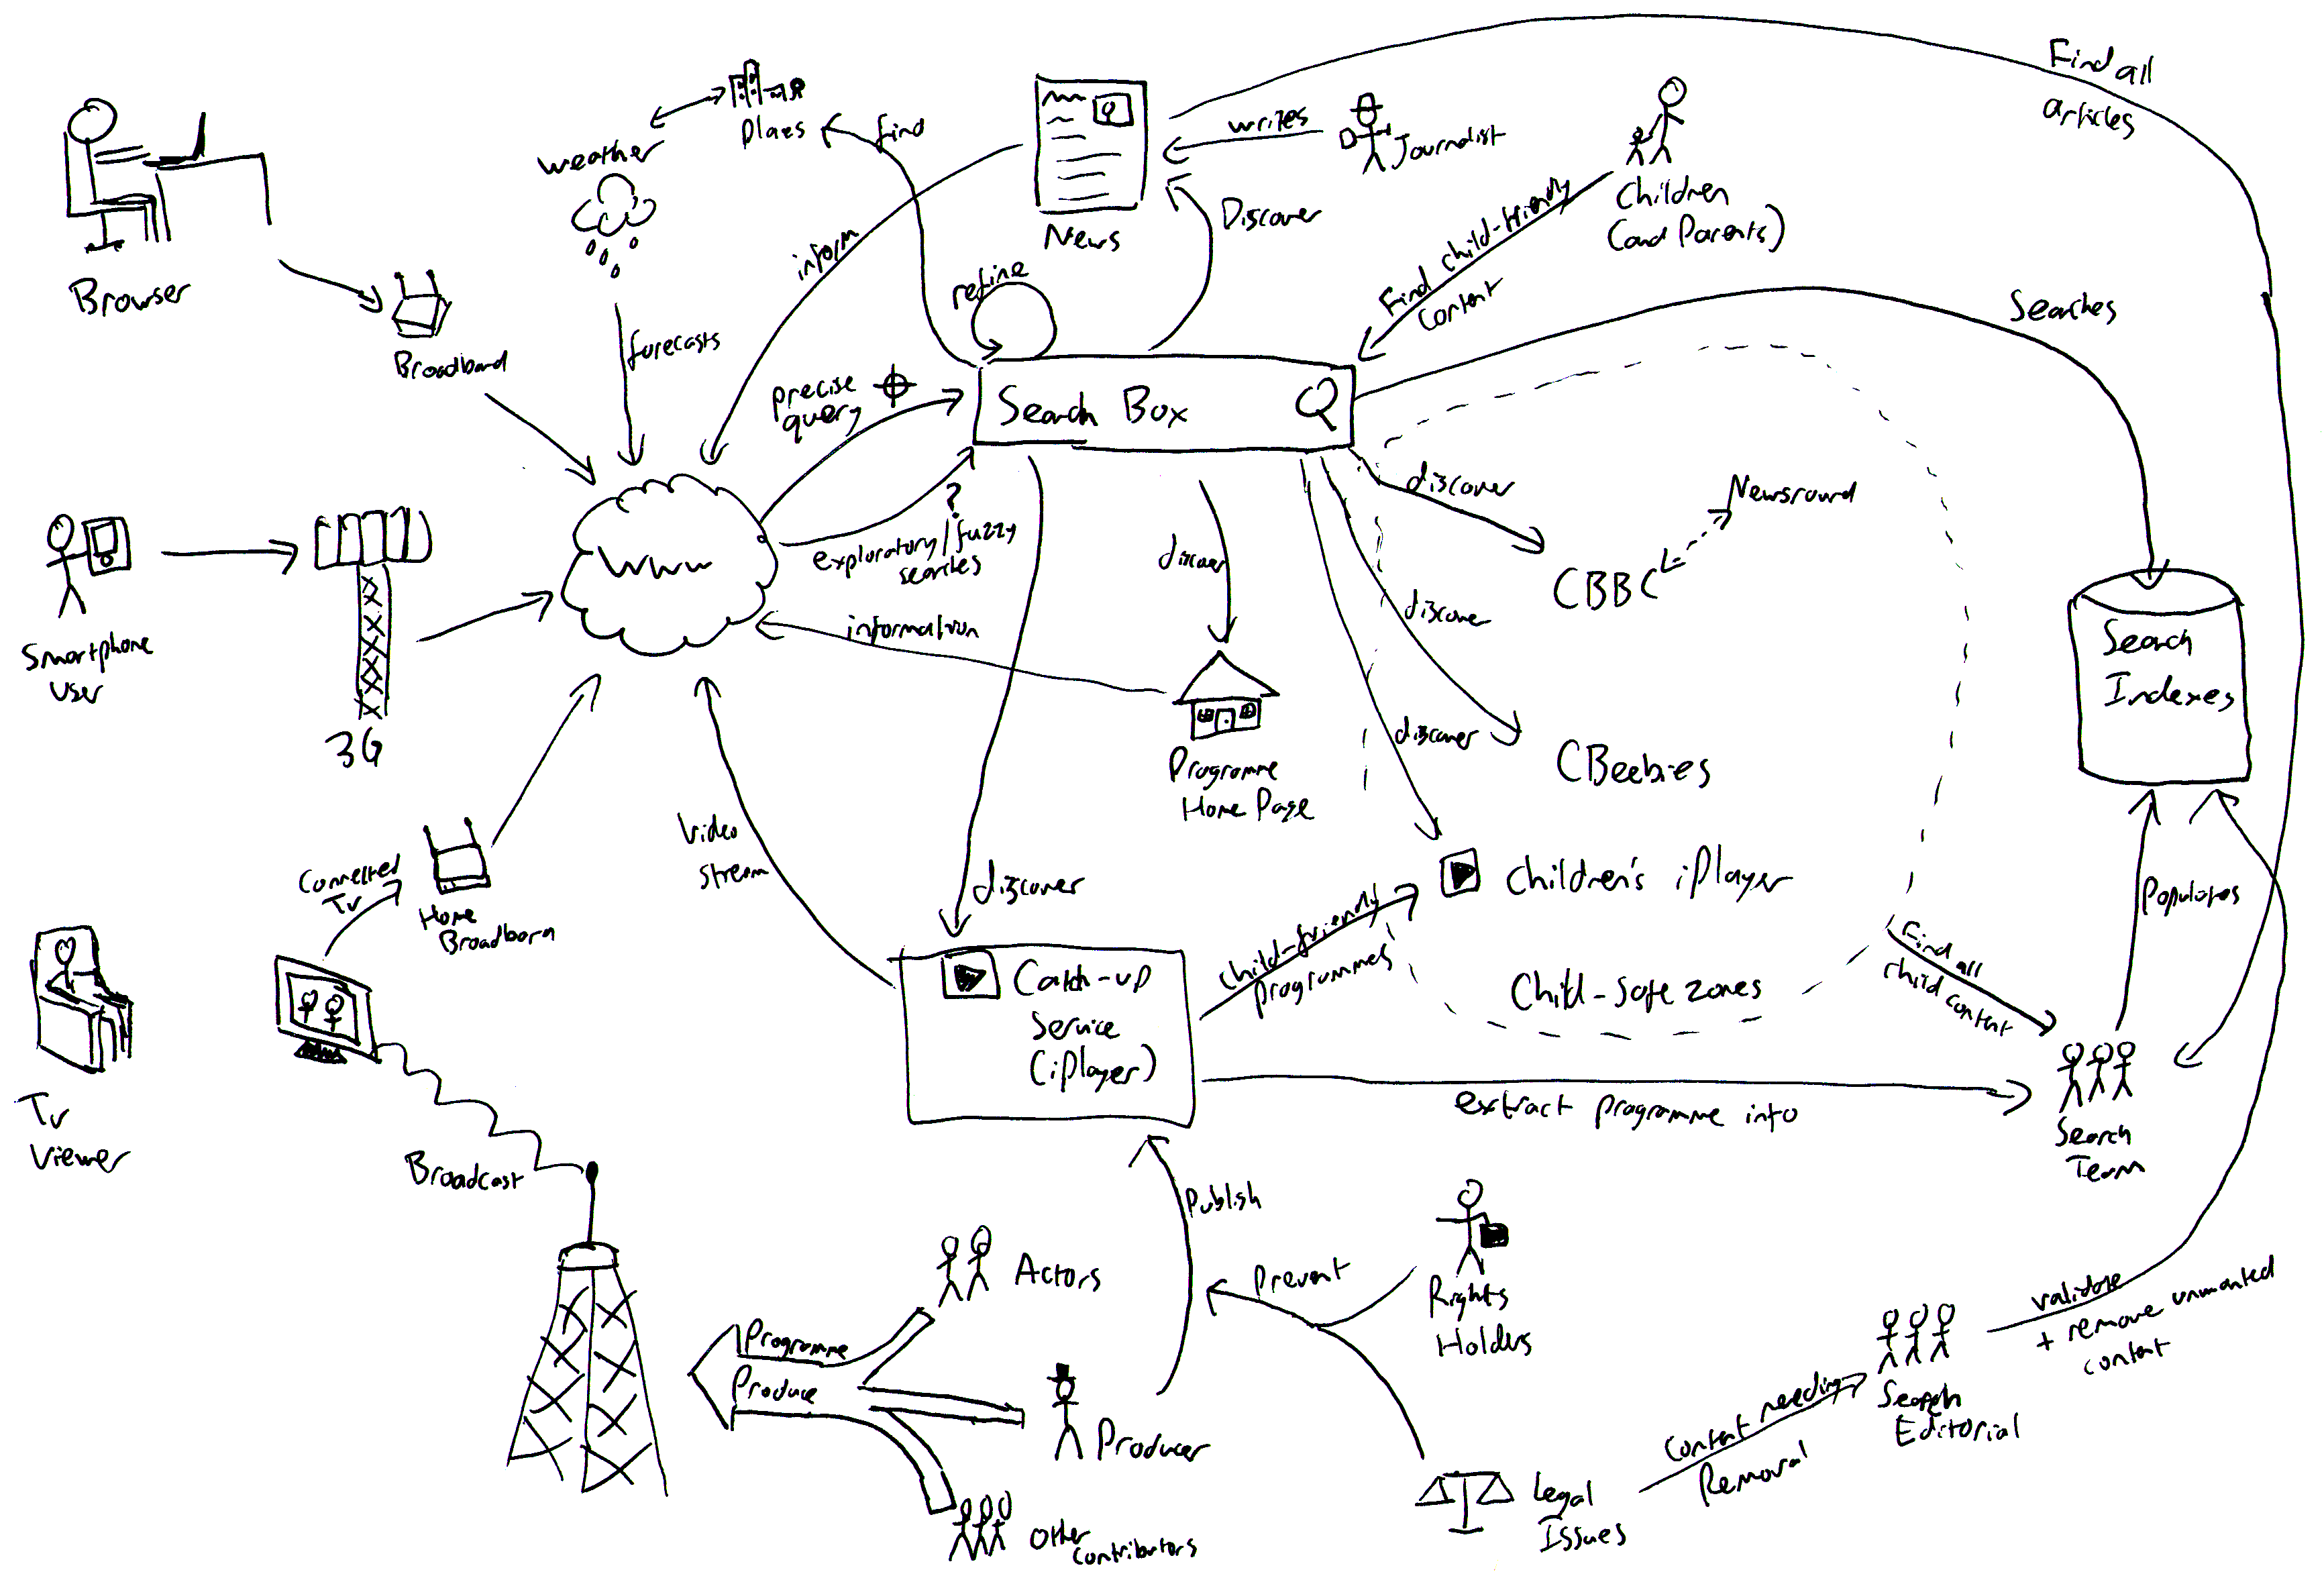
\includegraphics[width=\linewidth]{rich-picture.png}
  \end{center}
  \caption{Rich Picture of the BBC search system\label{rich-picture}}
\end{sidewaysfigure}

\section{Design}
\label{design}

\subsection{Use Cases}

From the rich picture in Fig.~\ref{rich-picture}, we
extracted the activities that are clearly within the remit of a search
application. For example, the ability for editorial staff to manage
the content of the search indexes sounds like a feature the search
application would provide. Conversely, television actors and other
contributors to a programme are likely to interact only within a television
production subsystem with a producer or content editor being responsible
for publishing information about the final production's broadcast and
availability for streaming online.

This is not to say that we can simply cross off certain elements from
our depiction of the problem because they do not directly interact
with the subsystem being designed. The \emph{systems thinking} approach
advocated by Checkland\cite{checkland1999systems} encourages us to
consider the irreducible properties of each system at each level
of abstraction. Thus we need to consider not only a search application
subsystem that solves specific problems for its immediate users, but
also an application that contributes to the desirable, emergent
properties of the BBC service as a whole.

In the specific example of television programming, we need to maintain
systems thinking throughout the design process to ensure that we
create a search application that both meets the needs of the public
using the application to search for programmes and forms part of
a television production and delivery system that itself meets the
needs of the television-watching public.

Thus a suitable design strategy is to apply systems design to
the search application in isolation -- as a \emph{hard problem} --
but then to use the wider system to inform, shape and evaluate that design.

Having extracted the activities that appear to pertain to the
search application directly (and the actors involved in those activities),
we can produce the use case UML diagram shown in Fig.~\ref{use-case}.

This illustrates only a subset of the expected behaviours for a full
BBC search application, but touches on some of the diversity of the
potential uses. For the purposes of our initial design, we can next look
into defining the system behaviour for some of these use cases.

\begin{sidewaysfigure}
  \begin{center}
    \includegraphics[width=\linewidth]{use_case.png}
  \end{center}
  \caption{Use case diagram for BBC Search application\label{use-case}}
\end{sidewaysfigure}

\subsection{System Behaviour}

\begin{comment}
@startuml plant_sequence_producer.png

skinparam monochrome true

actor Producer
participant "Programmes Database" as prog
participant "Search Index Service" as service
participant "Search Indexes" as indexes

Producer ->> prog

activate prog
prog ->> service
deactivate prog

activate service
service ->> indexes
deactivate service

activate indexes
indexes -> indexes : reindex
deactivate indexes

@enduml
\end{comment}
\begin{figure}[t]
  \begin{center}
    \includegraphics[width=\linewidth]{plant_sequence_producer.png}
  \end{center}
  \caption{Sequence diagram showing publication of programme information to the search indexes\label{sequence-producer}}
\end{figure}

\begin{comment}
@startuml plant_sequence_user.png

skinparam monochrome true

actor User
participant "BBC Website" as www
participant "Search Service" as search
participant "Search Indexes" as indexes
participant "Source Service" as source

User -> www : types query into search box
activate www

  www -> search
  activate search

    note over search
      The service may want to vary the
      query for a number of reasons such
      as the type of device the user has
      or the nature of the query itself.
    end note

    search -> search : decide query parameters

    search -> indexes : raw query
    activate indexes
    indexes --> search : list of matching items
    deactivate indexes

    loop for each item
      search -> source : Fetch more info about item
      activate source

      note right of search
        We can enrich the retrieved items with
        more information from the original source
        systems rather than replicate all domain
        knowledge in the search indexes.
      end note

      source --> search : Returns richer info
      deactivate source
    end

  search --> www : list of enriched results
  deactivate search

www --> User : search results page
deactivate www

@enduml
\end{comment}
\begin{figure}[p]
  \begin{center}
    \includegraphics[height=0.4\textheight]{plant_sequence_user.png}
  \end{center}
  \caption{Sequence diagram showing a user interacting with search\label{sequence-user}}
\end{figure}

\begin{comment}
@startuml plant_sequence_ajax.png

skinparam monochrome true

actor User
participant "BBC Website" as www
participant "Search Service" as search
participant "Search Indexes" as indexes
participant "Source Service" as source

User -> www : types query into search box
activate www

  www -> search
  activate search

    note over search
      The service may want to vary the
      query for a number of reasons such
      as the type of device the user has
      or the nature of the query itself.
    end note

    search -> search : decide query parameters

    search -> indexes : raw query
    activate indexes
    indexes --> search : list of matching items
    deactivate indexes

    search --> www : Return stub items
    deactivate search
    
    www --> User : search results page

    note over www
      Website remains active using Javascript to do 
      AJAX requests for further information for
      each result.
    end note

    loop for each item
      www ->> search : Fetch more info about item
      activate search
      search -> source : Proxy to source for info
      activate source
      source --> search : Return info in source's own format
      deactivate source
      search --> www : Return info in common format
      deactivate search
      www --> User : Update page in front of user as info arrives
    end

deactivate www

@enduml
\end{comment}
\begin{figure}[p]
  \begin{center}
    \includegraphics[height=0.4\textheight]{plant_sequence_ajax.png}
  \end{center}
  \caption{Sequence diagram showing rich information lazy-loaded via AJAX\label{sequence-ajax}}
\end{figure}

Figure~\ref{sequence-producer}
shows how a TV producer indirectly interacts with search by providing
information that ultimately ends up in the search indexes and
Fig.~\ref{sequence-user} shows a sequence diagram defining a user
interacting with the search system

The key design decision in Fig.~\ref{sequence-producer} is the use of
asynchronous messages only. A non-blocking set of interactions such as
publish-subscribe\cite{hohpe2004enterprise} is a good way to decouple
systems that produce and store progamme information from the search
application systems. If the systems surrounding the programmes database
can be built a \emph{channel adapter}\cite{hohpe2004enterprise} to integrate
it to a messaging system, then the search indexes can receive changes to
information without TV producers, journalists, content
editors, etc. even being aware this is happening.

Note in Fig.~\ref{sequence-user} that while the search indexes
will contain representations of content
from several source systems, the intention shown is that richer information
about the domain model will not be held in the search indexes. This goes
along with the principle of separation of concerns\cite{dijkstra1982role}
in that the search index component can focus on optimising its data
structures around retrieval. This kind of modularity also allows source
systems maintained by other teams to take the responsibility of the
accuracy of the information, which fits in with the wider holistic view
of the system: the volume of information involved requires that
separate teams are responsible for the accuracy of their data.

This can be seen as similar to the \emph{Lazy Load} pattern
\cite{fowler2002patterns} in that the search indexes will only return
stub objects that are capable of retrieving the fuller information
to need. This, however, could lead to a lot of calls to different
service applications per page of results. This can be done in parallel, but
the fact still remains that the user has to wait for all this to
assemble before seeing even one result.

One solution to this in modern web application design is to
push the lazy loading into the web browser using AJAX\cite{garrett2005ajax}.
Such a solution is depicted in Fig.~\ref{sequence-ajax}. Whilst
this still requires just as many calls to backend services --
perhaps even more complexity as the calls are going through
more layers -- it can give a user experience that appears more responsive.

Preparing a search results page with minimal information that is then
augmented asynchronously is a user experience technique that gives the
illusion of lower latency; the additional information can update the page
during the user's reaction time in the best case.

\subsection{Domain Model}

It has been expressed already that a BBC-wide search application
would need to index, retrieve and display a diverse set of
information. Parts of the application might well want to incorporate
a domain model\cite{fowler2002patterns} so as to understand how
to perform each of these actions against each possible item
the search application could return as a search result.

Domains are the distinct subject matters present in any system
representing large, reusable components and are depicted using a
domain model which shows an organisation of UML packages and their
dependencies\cite{dickerson2009architecture}. The use case diagram and domain model
developed provides a baseline model for a future search application system.

A maximal
domain model is shown in Fig.~\ref{model} that attempts to capture
a good proportion of the content and concepts the BBC has
been making efforts to model over several years. This model is
an aggregate of individual ontologies developed for specific purposes,
but given the search application has to provide the discovery for
the full set of this information, it is not unreasonable that
a search application would have a domain model that covers the totality.

Note that complexity of information for programmes alone\cite{raimond2009bbc}.
A programme to a member of the public could actually refer to an
exact episode or indeed the \emph{brand}, i.e. the title of the programme
in general. An example of a brand would be
\emph{Doctor Who},
\footnote{\emph{Doctor Who} is a popular, long-running science-fiction
television programme produced by the BBC and is frequently sought by users
of the BBC iPlayer television catch-up service after an episode has aired.
} which itself contains multiple series, which in turn
contain a collection of episodes. Note that the brand itself has episodes
as immediate children that do not live under a series, e.g. Christmas specials.
It is also the case that certain things do not have brands or series, e.g.
a film is modelled as a one-off episode.

This leads to some difficult questions for a search application. If a user
searches for the text ``doctor who'',
are they expecting a link to the
latest episode to watch on iPlayer, information about the next episode
-- such as when it is due to be broadcast -- or a link to the overall
home page for the entire Doctor Who brand?

The model also skims the surface of the sport ontology\cite{rayfield2011bbc}
created before the 2012 Olympic games, which aims to model the whole domain
of sporting personalities, events and competitions (and more). This might
be too fine-grained for the domain model used within the search application,
but it is likely that people will want to search for competitions like
``World Cup'' or sporting disciplines such as ``football''. A search application
that understands these concepts as entities in their own right may well
be able to direct users at a curated, dedicated ``home page'' thereof alongside
simply matching articles and other works that contain those terms.

\begin{comment}
@startuml plant_model.png

skinparam monochrome true
skinparam circledCharacterRadius 0
skinparam circledCharacterFontSize 0


package CreativeWorks {
class CreativeWork {
  title : String
  dateModified : DateTime
  dateCreated : DateTime
  category : String
  description : String
  thumbnail: Image
}
class NewsItem extends CreativeWork
class BlogPost extends CreativeWork
class LiveCoverage extends CreativeWork
class LiveEventPage extends CreativeWork

interface Format
class TextualFormat extends Format
class VideoFormat extends Format
class InteractiveFormat extends Format
class ImageFormat extends Format
class AudioFormat extends Format
class PictureGalleryFormat extends Format
}

package Programmes {
class Programme
Programme -r-|> CreativeWork
class Brand extends Programme
class Series extends Programme
class Episode extends Programme

class Service
class Version
class Broadcast
class Ondemand
}

Service "1" -- "0..n" Programme : masterBrand
Episode "1" *-- "0..n" Version : hasVersions

Version "1" -- "0..n" Broadcast : broadcasts
Version "1" -- "0..n" Ondemand : availableOndemandWindows

Broadcast "1..n" -- "1" Service : broadcastOn
Ondemand "1..n" -- "1" Service : availableOn

Brand "1" *-r- "0..n" Series
Series "1" *-d- "0..n" Series
Series "1" *-r- "0..n" Episode

package Concepts {
class WebDocument
class Thing {
  preferredLabel
}
class Person extends Thing
class Event extends Thing
class Place extends Thing
class Theme extends Thing
class Organisation extends Thing
}

CreativeWork "1" -- "1..2" WebDocument : primaryContent
Thing "1" -- "0..n" WebDocument : primaryTopic
CreativeWork "0..n" -- "1" Format : primaryFormat
CreativeWork "0..n" -- "0..n" Thing : tag
Thing "0..n" -- "0..n" Thing : notablyAssociatedWith


package Sport {
class SportCompetition extends Event
class SportDiscipline extends Thing
}

Event "0..n" -- "0..n" Programme : coverage
SportCompetition "0..n" -- "0..n" Person : competesIn
SportDiscipline "1" -- "0..n" SportCompetition

@enduml
\end{comment}
\begin{sidewaysfigure}
  \begin{center}
    \includegraphics[width=\linewidth]{plant_model.png}
  \end{center}
  \caption{Domain model for content items and other things pertinent to BBC content\label{model}}
\end{sidewaysfigure}

\subsection{Discussion and Analysis}
\label{appraisal}

The problem of
a BBC-wide search application was predicted --
and has certainly shown itself -- to be a very large-scale problem, the
full extent of which cannot be covered in this paper. Thus it
is reasonable to conclude that the problem is not yet solved
at every level, but the high-level solutions are certainly promising.

The use case diagram is likely not complete and would need
a significant amount of user research and requirements-gathering
to collect all the possible use cases of the search system. It
is likely that the variations of the use cases are so numerous
that different diagrams exploring different combinations of use
cases should be made to replace the single one given. For instance,
very little has been touched on around users seeking educational
and informative material such as \emph{Bitesize}
\footnote{\emph{Bitesize} is the name given to the BBC's free web-based
study materials for school children aged between
5 and 16, covering varying curricula for England, Wales and Scotland.}
or any other learning resources.

The sequence diagram for the producer (or any other content creator)
indirectly getting their content into the search system demonstrates
the need for asynchronous messaging (and publish-subscribe), but
the nuances of such a process are not comprehensively shown in
this format. A better illustration for such a message-based integration
system might be derived from the illustrated patterns created
by Hohpe and Woolf\cite{hohpe2004enterprise}.

The behaviour of the query web application in Fig.~\ref{sequence-user}
is defined with a hard line
taken on keeping the information stored in the indexes to a minimum.
At a basic level, this is not unlike a \emph{content enricher} pattern
\cite{hohpe2004enterprise} whereby the search application
business layer enriches the stubs in the indexes with information
the source system (the index) simply does not have. At a more purist
extreme, this could follow a \emph{claim check} pattern where
the index returns only globally-unique identifiers for the matching
items and makes no attempt to present any other knowledge about them
(and thus avoids any synchronisation issues if an item is updated at
source).

The latter pattern fully decouples the search indexes from any
deeper information -- leaving that responsibility to appropriate
source system -- but means that the raw, stub results are near-useless
to an end user. This makes the AJAX-based alternative approach
in Fig.~\ref{sequence-ajax}
less of a desirable option (would a user really be presented a list
of URIs while some Javascript code replaces them one by one with
actual information?). Given the AJAX-driven behaviour still appears
desirable in terms of responsiveness, it would seem that some trade-off
would need to happen in terms of what the indexes store as additional
information.

These decisions relate to how the system would implement the data model
in Fig.~\ref{model}. The ontology described is an aggregation
of several efforts by Raimond\cite{raimond2009bbc}, Rayfield
\cite{rayfield2011bbc} and others -- along with some additional work
to join them together -- to represent the wealth of
information with which the BBC deals. It could be argued both that
a search application that \emph{understands} this diversity of
content must reflect it in its domain model but that a search
application that is \emph{coupled} to the individual ontologies
in this way is brittle with regard to changes therein. Duplication
of business models across different applications would only
harm maintainability.

Thus the domain model given in Fig.~\ref{model} should only serve
as a communication artefact that leads to further development of
a domain model more suitable to the needs of the search application
without the burden of maintaining more than is necessary. The use
of \emph{subtype polymorphism}\cite{booch2007object} is likely
to be key to ensure the search domain model contains only the APIs
it needs. For example, does the search application have a need
to differentiate between a \emph{NewsItem} and a \emph{BlogPost}
for the purposes of displaying the search result's title? If the
CreativeWork top-level class has a title property, then the domain
model so far to enable that one behaviour needs only one class!

The application could go further and interact via a single
SearchResult \emph{facade}\cite{fowler2002patterns} whose
instances provide appropriate responses to canonical hooks
such as \emph{getDisplayTitle()} and \emph{getDestinationUrl()}
via polymorphic \emph{composition} with different target classes
from the fuller domain model. Given that the search indexes
are likely to take in content from any number of future systems,
there is an appeal to taking a schemaless approach\cite{sadalage2012nosql}
and allow the search application's view layer to display
different kinds of results differently via \emph{duck typing}
\cite{python2013ducktyping}.

A dynamic, schema-free domain model used within the search application
-- noting that, of course, schemaless truly means there is an
implicit schema in the logic that creates these dynamic objects from
source systems\cite{sadalage2012nosql} -- could prove to aid the
search system's need to model different kinds of data in the same
index. For example, our designers might express a desire to put
small summaries of weather forecasts within search results that
contain places. In the static sense, we could say that anything
of \emph{Place} type is displayed with such a feature. With
a dynamic, duck-typed model, we could ask
``does this item have weather?'' in place of ``is this a place?'', thus
allowing for the future design that extends forecasts to football
matches (since football matches are \emph{Event}s that occur in
a \emph{Place}, it is reasonable for a weather property to be
set thereon).

Overall, we have some promising, high-level models from which to
start making such more fine-grained decisions about the search
application. The use cases are likely sufficient for early iterations
or a \emph{Minimal Viable Product}\cite{junk2000dynamic} and
the behaviours capture the overall needs of the system. There is still
much scope for returning to our systems thinking and Soft Systems
Methodology to monitor the general model for Checkland's ``3 Es''
(efficacy, efficiency and effectiveness)\cite{checkland1990soft},
which is only briefly touched on in the authors' attempts to relate the
data model to the user's interaction with the system.

\section{Evaluation}
\label{evaluation}

The high-level nature of the modelling achieved has made it
difficult to meet any objectives over performance, latency or
robustness of software components involved. A BBC search application
needs to index news as it is published, serve millions of unique
visits every week and minimise potential for losing information. These
non-functional requirements are a challenge in their own right
and have not been met with the UML modelling presented.

This is not to say that UML is not capable as a tool for presenting
architecture around performance and resilience. However, it is perhaps
more appropriate to model and present some of these aspects through
component and deployment diagrams. Behaviour diagrams such as sequence
and activity do not suit well to showing timing or performance, although
a series of sequence diagrams could show how behaviour changes
in parts of the system to tolerate failure of other components (e.g.
one component could be modelled to return from an internal cache if
a collaborator is returning temporary error status codes).

Even the models that are presented in this paper do not paint the full
picture, but it could be argued that it is not their purpose to do so.
As stated at the end of Sect.~\ref{appraisal}, the use case diagram
provides a starting point that might be sufficient for an early
iteration of a project in an \emph{Agile} methodology\cite{beck2001agile}.

An Agile approach to developing the search application could distill
the use cases even further and shape the requirements to the rest
thereof later in the development process based on feedback and reacting
to changes. A similar approach would allow us to start with the smaller
domain model also discussed in Sect.~\ref{appraisal} and allow it to grow
to the necessary size to need -- i.e. we can defer the decision of ``how big
should the domain model be?'' until we are at a point where we have more
information to answer such a question.

Thus even if the use case and domain models are not as comprehensive or
as honed as they need to be to build an entire application, they serve
their purpose adequately to communicate the first iterations of
development or -- especially in the case of the domain model -- information
pertaining to the whole organisation, even if only small parts of it are
they modelled directly in the application being built.

The sequence diagrams seem to provoke more debate of the merits of
returning rich information in a single response versus an AJAX-driven
approach (or some trade-off in between). Again, the authors would emphasise the
communication aspect of UML modelling and argue that encouraging such debate
is a successful application of UML, not a failure because a decision
has not been made between two designs at this early stage.

Some of this hints at a drawback of UML modelling being that it encourages
a lot of design decision at an early stage of a project -- a stage at which we arguably
have the least information\cite{kelly2013conway}. However, there are plenty of
efforts in spite of this that promote modelling and UML being used
compatibly within an Agile process. The use of other modelling techniques
in an Agile setting such as
Rational Unified Process (RUP) and Agile Unified Process (AUP) have been
suggested as suitable in an Agile project\cite{ambler2002agile}.
 It may have been more suitable to incorporate
a more diverse range of modelling techniques in the design and analysis
presented so as to find the true strengths of each respective approach.

In conclusion, the UML modelling presented communicates some promising
approaches to
the BBC search problem, but it is far from sufficient in its own right.
Designing to the level of detail required would result in a rigid
development plan that made unverified assumptions, but an iterative
approach to modelling that starts at a high-level and updates as
development progresses could be used successfully in such a project.

A post-analysis study is required to evaluate the SSM and UML models. The models
need to be applied to further projects for validation and verification purposes.
In addition, the maturity and evolution of the artefacts need to be considered
e.g. adding, deleting, or modifying, if the boundary and context changes.

\bibliographystyle{splncs}
\bibliography{bibtex}

\end{document}
